\chapter{Vizuál stránky}

Úvodná stránka index.php ktorá je jednoduchého designu, s Headerom\footnote[1]{Element <header> HTML predstavuje úvodný obsah, zvyčajne skupinu úvodných alebo navigačných pomôcok. Môže obsahovať niektoré prvky záhlavia, ale aj logo, vyhľadávací formulár, meno autora a ďalšie prvky.}, ktorý sa opakuje na každej podstránke, nás privíta krátkym textom ktorý momentálne nahrádza text Lorem Ipsum. Stránka má v Headery umiestnené logo SF ktoré je viditeľné aj v náhľade stránky, v lište prehliadača. Toto logo funguje taktiež ako odkaz, ktorý nás pri kliknutí, vždy premiestni na úvodnú stránku index.php. V spodnej časti stránky sú umiestnené 2 hypertextové odkazy na LinkedIn a email. Úvodnú stránku môžeme vidieť na obr.\ref{OBRAZOK 1.1}

\begin{figure}[!tbh]
\centering
\setlength{\fboxsep}{0pt}%
\setlength{\fboxrule}{1pt}%
\fbox{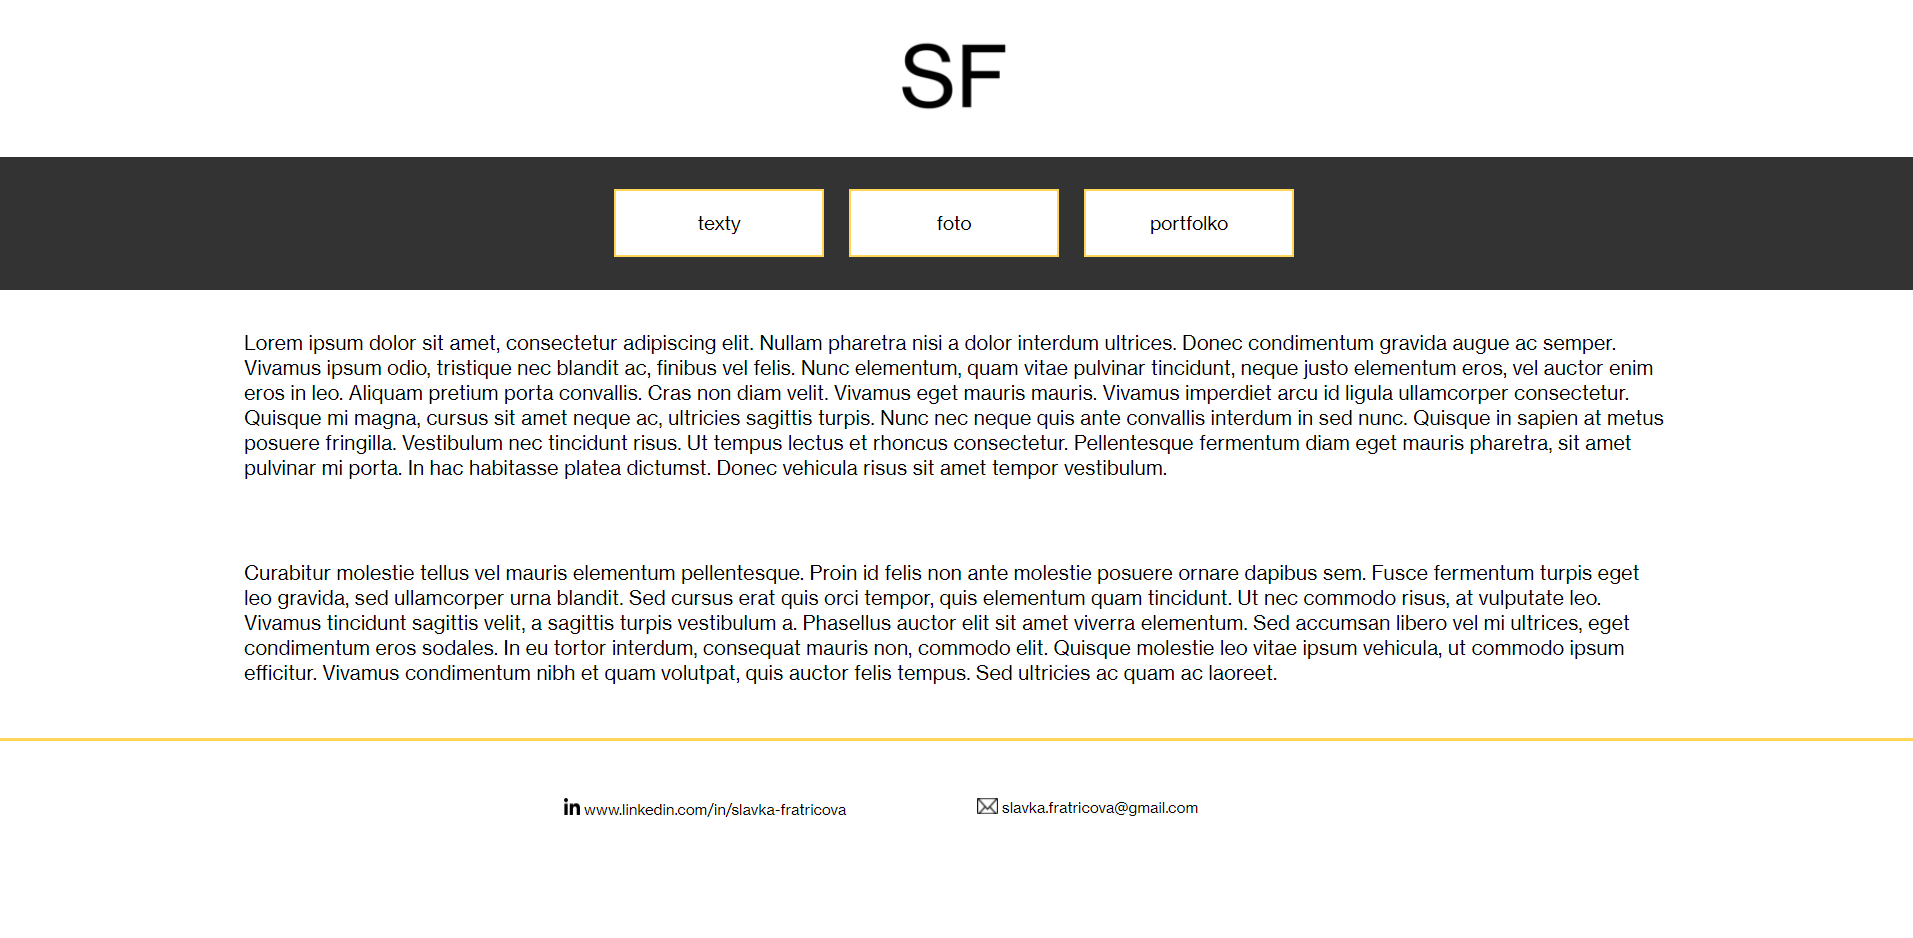
\includegraphics[width=\textwidth]{obr/uvodka.png}}
\caption{Úvodná stránka index.php.}\label{OBRAZOK 1.1}
\end{figure}






